% Candidate schematic; a^2=b^2+c^2, b>c>0. Coordinates use c=1,b=1.3.
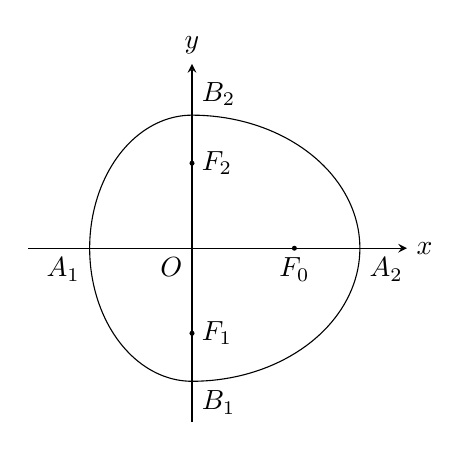
\begin{tikzpicture}[scale=1.3,>=stealth]
\draw[->] (-1.6,0)--(2.1,0) node[right] {$x$};
\draw[->] (0,-1.7)--(0,1.8) node[above] {$y$};
\draw plot[domain=-90:90,samples=81] ({sqrt(2.69)*cos(\x)},{1.3*sin(\x)});
\draw plot[domain=90:270,samples=81] ({cos(\x)},{1.3*sin(\x)});
\fill (1,0) circle (.7pt) node[below] {$F_0$};
\fill (0,{sqrt(.69)}) circle (.7pt) node[right] {$F_2$};
\fill (0,{-sqrt(.69)}) circle (.7pt) node[right] {$F_1$};
\node[below left] at (0,0) {$O$};
\node[below left] at (-1,0) {$A_1$}; \node[below right] at ({sqrt(2.69)},0) {$A_2$};
\node[below right] at (0,-1.3) {$B_1$}; \node[above right] at (0,1.3) {$B_2$};
\end{tikzpicture}
